
%--------------------------------------------------------------------
%--------------------------------------------------------------------
% Formato para los talleres del curso de Herramientas Computacionales
% Universidad de los Andes
% 2015-10
%--------------------------------------------------------------------
%--------------------------------------------------------------------

\documentclass[11pt,letterpaper]{exam}
\usepackage[utf8]{inputenc}
\usepackage[spanish]{babel}
\usepackage{graphicx}
\usepackage{mdframed}
\usepackage{tabularx}
\usepackage[absolute]{textpos} % Para poner una imagen completa en la portada
\usepackage{multirow}
\mdfdefinestyle{mystyle}{leftmargin=1cm,rightmargin=1cm,linecolor=red}
\usepackage{float}
\usepackage{hyperref}
\decimalpoint
%\usepackage{pst-barcode}
%\usepackage{auto-pst-pdf}

\newcommand{\base}[1]{\underline{\hspace{#1}}}
\boxedpoints
\pointname{ pt}
%\extrawidth{0.75in}
%\extrafootheight{-0.5in}
\extraheadheight{-0.15in}
%\pagestyle{head}

%\noprintanswers
%\printanswers
\renewcommand{\solutiontitle}{}
\SolutionEmphasis{\color{blue}}

\usepackage{upquote,textcomp}
\newcommand\upquote[1]{\textquotesingle#1\textquotesingle} % To fix straight quotes in verbatim

\begin{document}
\begin{center}
{\Large Herramientas Computacionales} \\
Taller 4 - \textsc{Python}:\\
Operaciones aritméticas, listas, condicionales, \newline cadenas de caracteres y estructuras iterativas. \\
Fecha de publicación: {\small \it Febrero de 2015}\\
\end{center}

\begin{textblock*}{40mm}(10mm,20mm)
  
\includegraphics[width=3cm]{logoUniandes.png}
\end{textblock*}

\begin{textblock*}{40mm}(161mm,20mm)
  
\includegraphics[width=3cm]{logoUniandes.png}
\end{textblock*}

\vspace{0.5cm}

{\Large Instrucciones de Entrega}\\

Los scripts de solución de este taller deben ser presentados en un solo archivo con nombre \verb+NombreApellido_HW4.zip+ en \textbf{sicuaplus}.

En cada parte del ejercicio se entrega 1/3  de los puntos si el código propuesto es razonable, 1/3 si se puede ejecutar y 1/3 si entrega resultados correctos. El script debe llevar comentarios suficientes.


\vspace{0.5cm}


\begin{questions}

\question[60] {\bf Imprimiendo en Espiral}
\begin{parts}
\part[40] Escriba un programa que toma como input un vector con los números de 1 a $n^2$ y que los imprima en una matriz cuadrada, de dimensiones $7x7$ en espiral en el sentido de las manecillas del reloj. El programa debe imprimir los números en pantalla, separados por un espacio. llamelo \verb+espiral_reloj.py+

\begin{center}
	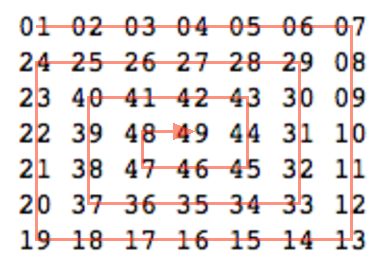
\includegraphics[width=0.2\textwidth]{./spiral7.pdf}
\end{center}

\part[20] Escriba un programa que haga lo mismo en el sentido en contra de las manecillas del reloj para una matriz cuadrada de $8x8$.
\end{parts}

\question[40] {\bf Palíndromos en inglés}
Escriba un script llamado \verb+palindromo.py+ que encuentre todos los palíndromos de una palabra \footnote{Definición de Palíndromo: \url{http://es.wikipedia.org/wiki/Palindromo}}. de la siguiente lista de palabras: \url{http://www-01.sil.org/linguistics/wordlists/english/wordlist/wordsEn.txt}. Imprima la lista de palíndromos en un nuevo archivo de texto llamado \verb+palindromos.txt+. Cuántos encontró?


\end{questions}


\end{document}
